\documentclass{llncs}
\usepackage{graphicx}
\usepackage{url}
\usepackage[utf8]{inputenc} % Umlaute (währinger straße)


\begin{document}

\title{Evaluation of a Visualization Component for the Difference Graph}
\author{Firstname Lastname \and Firstname Lastname}
\institute{Universität Wien \\ Währinger Straße 29 \\ 1090 Wien}
\maketitle
\begin{abstract}
Finding differences between two processes can be a complex, time consuming and expensive task. Our work is based on the difference graph which calculates the differences of two process models. We want to extend the model with and expressive visualization to show where differences can be found. In order to find the best suiting visualization we extracted several visualizations from literature. These visualization were the foundation of an evaluation. The result showed that color coding suits the difference graph visualization best.
\end{abstract}

\begin{keywords}
	Difference Graph, Visualization
\end{keywords}


%Todo:
% Update Images -> Resolution, Font and Visuals
% Read everything

\section{Introduction}
\label{sec:Introduction} % [1 Page]

Processes are an indispensable part of today’s business. From visualizing processes for communication, up to optimization we constantly use processes to gain additional business intelligence.

%What is the problem / how is it solve by now
Using process mining algorithms on data collected during process execution allows further analysis \cite{lit:PMDiscoveryConformanceEnhancement}, for example, detection of bottlenecks, problems and violations. Conformance checking \cite{lit:ConformanceCheckingOfProcesses} is a part of process mining which allows to check if a log file deviates from a process model. Unfortunately conformance checking focuses only on detection of deviations between log files and process models. With their paper \cite{lit:VisuApprDiffAnalysis} introduced the difference graph which allows to check for differences between two process models. These models can be generated through process mining or even crafted by hand. 
However they do not evaluate how to visualize the difference model. Visualizing data is a very important task to enhance the users understanding of the data. 

%Contribution
In this work we investigate the following research question: Which visualization suites the difference graph best? To answer this we conduct a literature research to find different representations. Afterwards we use a survey to evaluate which of the found visualizations should be used for representing the difference graph.

%Applications
Difference calculation and visualization can be used in different areas of application. One is to compare process models generated with process mining techniques from two processes. This helps finding deviations between those processes. For example, a company with two locations executes the same task. Unfortunately in one location the execution takes twice the time. Comparing the process models of these locations can help finding why the execution time is doubled. When comparing two process models one can although gain additional information if those processes can be merged. Finding deviation allows to determine where problems may occur. Another area of application is to use one process at different points in time. For example, compare the years 2013 and 2014 of one process. This allows to see how the process has evolved.

%Section overview
In Section 2 we give an overview of the difference graph model and calculation. As well as an outline why the visualization is important. To select an appropriate visualization Section 3 covers our evaluation process. Related work can be found in Section 4. Section 5 concludes this paper with a reference where future work can be done.



%\textit{Literature to solve this problem}
%Current process mining methods are able to check for compliance (check rule violation while or after the process is executed) and conformance (compare a log with a process model).
%In some cases it is not useful to compare real world process logs with handcrafted process models. What if two real world processes should be compared?
%This question answer \cite{lit:VisuApprDiffAnalysis} with the introduction of their difference graph model. They presented the model and essential parts for calculation. However they do not evaluate how to visualize this model. Visualizing data is a very important task to enhance the users understanding of the data.


\section{Difference Graph Model and Visualization} % [2 Pages]
\label{sec:DiffgraphModel}
The difference graph concept \cite{lit:VisuApprDiffAnalysis} consists of two parts one is the model and the other is the visualization of this model. In this section we will  first describe the difference model and then take a journey towards visualizing this model.

Elementary component for the difference graph model is a process model. According to \cite{lit:VisuApprDiffAnalysis} a process model is defined as a direct connected graph \textit{PM} = (\textit{N}, \textit{E} $\subseteq$ \textit{N} $\times$ \textit{N}). \textit{PM} consist of nodes \textit{N} and direct control edges \textit{E}. Each node consists of an unique identifier, label and a type.
The process model consists of one start node which has no incoming edges and one end node which has no outgoing edges. Except from start and end node each node is connected by at least one incoming and outgoing edge. Every node has to be on a path between start and end node. Figure \ref{fig:ProcessModels} shows two process models. Input1 consists of four weighted edges and four labeled nodes. Input2 consists of three edges and although four labeled nodes. Interesting examples for difference calculation of these two inputs are node C where the weight has increase from 2 to 3, node B and E which are only visible in one of the inputs.

\begin{figure}
	\centering
	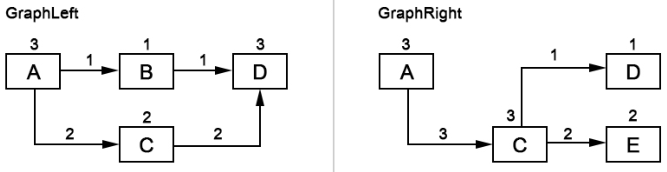
\includegraphics[width=0.8\textwidth]{Images/ProcessModels.PNG}
	\caption{Two process models.}
	\label{fig:ProcessModels}
\end{figure}

%Grafik anpassen *Input1, *input2 und Schriftart ändern

For generating the difference graph two process models are needed. These models can be described in many different process modeling languages e.g. Petri Nets \cite{lit:Petrinet}, UML \cite{lit:UML}, EPC \cite{lit:EPC}. All of those languages which are conform to the above mentioned process model description can be used for the difference graph calculation. From both input process models the difference graph model is calculated. This model extends a process model with an element called marking. The marking is applied on edges and nodes and is generated during the calculation process.

%Noch auf die Unterschiede eingehen? ein Difference Model kann bsp. mehr wie einen start/endknoten haben

For calculating the markings the first model is subtracted from the second one. During the calculation three or five different markings can be generated. Five markings can be calculated if the input process models consist of weights. If not, only three markings can be calculated. The following list shows all five markings and gives a description in which case they are used. 

\begin{itemize}
	\item \textbf{New}, a node/edge gains the marking New when the node/edge was added from Input1 to Input2.
	\item \textbf{Positively changed}, a node/edge is marked as Positively changed when the weight has increased from Input1 to Input2.
	\item \textbf{Unchanged}, a node/edge gains this marking when its value matches in both inputs.
	\item \textbf{Negatively changed}, a node/edge is marked as Negatively changed when the weight has decreased from Input1 to Input2.
	\item \textbf{Deleted}, a node/edge gains the marking Deleted when the node/edge was deleted from Input1 to Input2.
\end{itemize}

Hint the markings positively changed and negatively changed can not be calculated if the input process models do not consist of weights.

Figure \ref{fig:DiffGraphCalculation} shows the results for subtracting Input2 from Input1 which were shown in Figure \ref{fig:ProcessModels}. Node B  was deleted from Input2 therefore, the marking deleted is applied the weight is calculated by subtracting 1 from 0 = -1. Node C was changed positively the weight has increased from 2 to 3.

\begin{figure}
	\centering
	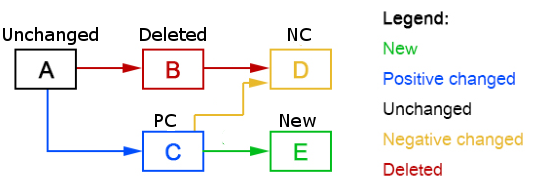
\includegraphics[width=0.8\textwidth]{Images/ResultGraph.PNG}
	\caption{Calculating the differences from Figure \ref{fig:ProcessModels} leads to this difference graph. On top of each edge and node calculated weights and applied markings are shown.
	%TODO: change all colors to Black and state on top of each node and edge which marking is applied. This will lead to the following: first the reader sees the two inputs, then he/she sees the calculation and later on in the evaluation he/she sees how this markings which are stated here with text are visualized.
	}
	\label{fig:DiffGraphCalculation}
\end{figure}

The main  focus of this paper is how to visualize the difference graph. The idea behind the visualization of the difference graph is to represent each of the markings with different styles. For example, each marking can be mapped to represent a specific symbol. This symbol can then be visualized on nodes and edges.

A survey was conducted to secure a good understanding of the difference graph visualization. To do so a literature research with the goal to find different visualization approaches was executed. Our first step was to find relevant keywords addressing the topic of difference visualization. These keywords where used within search engines. This led to a wealth of papers which where used as a basis for snowballing method where on one side other relevant papers where collected and on the other side new keywords where extracted. From all collected papers we were able to extract nine visualization approaches. These nine approaches were used in our evaluation.

This section gave an overview about the fundamental process model which is the base for the difference graph model. We showed how the difference graph model is calculated and which markings can be expressed on edges and nodes. For visualizing the model an appropriate style for markings has to be found which will be part of the next section.

\section{Evaluation} %  [5 Pages]
\label{sec:Evaluation} % [1/2 Page]
To address the research question, stated in Section 1, an online survey was conducted. Traditional ways like literature research and aggregation of information did not lead to an answer to our research question. However, we used the information found with literature research as input for our survey. The survey should show from the nine styles we found which of them fits the difference graph visualization best.


\subsection{Design} % [1/2 Page]
\label{sec:Design}
To avoid massive scrolling and simplify navigation through the survey we used single pages. Single pages come with the advantage that on each commit of a page we are able to validate the answers and give hints to the user where answers are missing. Overall the survey is divided into three groups introduction, styles and advanced/demographic questions.

The introduction gives an example how the difference graph is calculated and asks the user a question specific to this example. This question allows to check if the user understood the example or not. Further questions on the introduction page check the attendees knowledge about graphs.

Following the introduction are the visualizations for the difference graph. Each visualization consists of five different styles. For example, the visualization color coding consists of the styles green, blue, black, orange and red. Each of this visualizations is presented on a single page and consists of two questions. A question to rate the expressiveness of the visualization and a question for intuitive understanding. The question for intuitive understanding asks the user to determine which style represents which marking. For example, the visualization shows a node which is colored red and the user has to select one of the five markings mentioned earlier in this paper.

In the advanced/demographic section we first ask the attendee to rank the styles according to their expressiveness. Ranking the styles after seeing all of them allows additional evaluations. Additional questions from this section are, for example, if edges and nodes should be represented with the same style or if the style of the difference graph should be determined by the size of the graph. The survey concludes with demographic questions e.g. age, gender, employment.


\subsection{Procedure} % [1/2 Page]
\label{sec:Procedure}
After finalizing the surveys design a two-sided pretest was conducted.

In the first pretest a discussion with two people took place where the overall question and answer wording was adapted to support the users understanding.

In our second pretest five attendees had to complete the survey and give advices what should be changed. During their survey they where encouraged to think aloud and ask questions. All their questions and comments where noted and analyzed after the pretest. After finishing the second pretests minor changes to answers where made. This changes should secure a better understanding and reduce the surveys duration.

After finishing the pretests the URL to the survey was distributed by E-Mail to 159 people working in companies and studying in universities. Additionally the URL was posted on Facebook addressing students. Overall 103 attendees opened the survey from whom 31 attendees finished.


\subsection{Results and Discussion} % [2-3 Pages]
\label{sec:Results}
In this section we focus on the results of the survey. First we show the results to side topics followed by the results to our main research question.

Before we go into details which representation should be used for the difference graph we want to show that the difference graph can be understood by novices as well as experienced persons. In our survey overall 61.3 \% of the attendees understood the concept by the very first example. Another analysis shows that astonishing 73.6 \% attendees with fundamental graph knowledge understood the example. In contrast, only 41.6 \% of the attendees without graph knowledge understood the example. This analysis shows that the concept can be understood within one example, however it is more likely to be understood by people which are familiar with the concept of graphs.

\begin{figure}
	\centering
	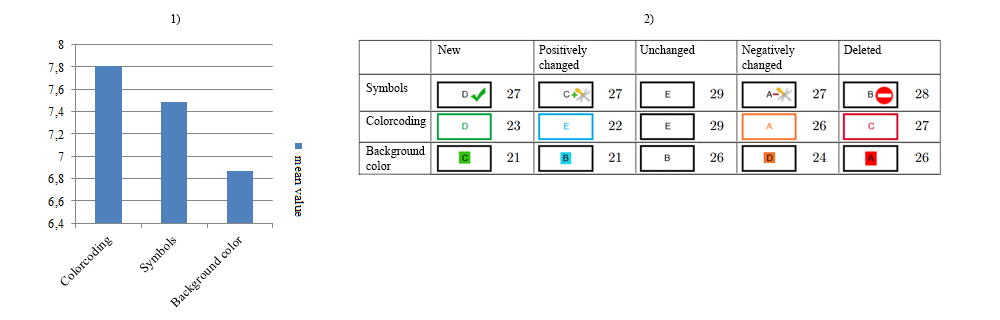
\includegraphics[width=350px]{Images/Results.PNG}
	\caption{SurveyResults}
	\label{fig:SurveyResults}
\end{figure}

To find the best suiting representation we analyze the intuitive understanding and the ranking for each style. The intuitive understanding is important to allow users to gain an overview of the visualization without the need to look which marking is represented by which style. The goal is to find a visualization where each style can be intuitively allocated to a marking.

Figure \ref{fig:SurveyResults}.1 shows a list of the top three visualizations in terms of intuitive understanding. On top of the list is the visualization "Symbols" followed by "Color coding" and "Background color". The maximum intuitive understanding possible is 31, which can only be achieved if every attendee assigns the same style to the marking. Symbols range from 27 to 29 with a mean value of 27,6. Means 27.6 attendees assigned the same marking to those symbols. For example, the green tick was assigned by 27 attendees as marking "New". Color coding has a mean value of 25,4 and "Background color" of 23,6.

After seeing all visualization approaches the users task was to order them according to their expressiveness. The ranking was transformed into numbers best ranking counts 9 worst 1. To compare the rankings the mean-value is calculated. Figure \ref{fig:SurveyResults}.2 shows the mean value for the top three representations. As before the figure shows the representations "Color coding", "Symbols" and "Background color". This time the order is different now "Color coding" is on top followed by "Symbols" and "Background color".

Within both evaluations only three of nine visualizations are on top. "Background color" was found in both evaluations on third place. Attendees commented that "Background color" is alike "Color coding" with the hint that "Color coding" is more useful then "Background color". Attendees mentioned "Color coding" is more pleasant to look at and more suitable for small as well as big graphs. While "Background color" is not suitable for big graphs. The reason for this is "Background color" only colorizes the label of a node. In big graphs finding the correct label for a node can be challenging. Therefore only the visualizations "Color coding" and "Symbols" are considered for further analysis.

Both visualizations offer advantages over the other. For "Symbols" the same negative aspect as for "Background color" can be encountered. Within big graphs finding the symbol assigned to a specific edge can be challenging. One solution would be to change visualizations with the size of the graph. Our evaluation showed that only 29 \% of attendees recommend to change the visualization with the graphs size.

We consider "Color coding" as the best visualization. The visualization offers a good intuitive understanding, scored best in the overall ranking and is suitable for small and big graphs. As commented by our attendees we recommend using a legend to show which color represents which marking.

Figure \ref{fig:DiffGraphVisualization} shows an example how the final representation can look. The figure shows the graph which was calculated in the previous example with applied color coding.

\begin{figure}
	\centering
	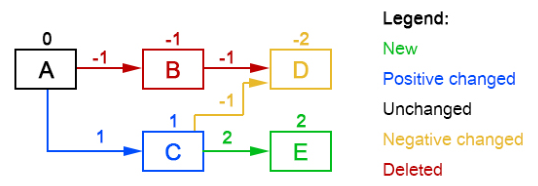
\includegraphics[width=0.8\textwidth]{Images/ColorCodedGraph.PNG}
	\caption{Color coded representation of the difference graph}
	\label{fig:DiffGraphVisualization}
\end{figure}

\section{Related Work}  % [1/2 Page]
\label{sec:RelatedWork}

Conformance checking \cite{lit:ConformanceCheckingOfProcesses} is a part of process mining \cite{lit:BusinnessProcessMiningAnIndustrialAppliction,lit:PMDiscoveryConformanceEnhancement} which deals with detection of inconsistencies between a process model and a log file. Conformance checking lacks of the possibility to compare two process models generated from log files. \cite{lit:VisuApprDiffAnalysis} proposed the difference graph concept where instance traffic of two processes is compared. They implemented a prototype where differences are visualized through color coding. They did not evaluate if color coding is a suitable option for visualizing differences within process models.

One of the first visualization approaches for process models where Petri Nets \cite{lit:Petrinet}. Since then many different languages emerged \cite{lit:YAWL,lit:UML,lit:EPC}. From process mining perspective the topic of visualization has also been addressed in \cite{lit:ProMFramework}. For the difference graph we need to show one process model which visualizes the differences of two process models. Therefore we extend previous work in this field by evaluating how differences can be visualized within process models.

\section{Conclusion} %  [1/2 Page]
\label{sec:Conclusion}
In our work we combine the difference graph concept with a visualization component. In the concept paper for the difference graph, color coding was mentioned as the preferred method for visualization. In our survey color coding was one of nine styles which can be used for difference visualization. Our evaluation confirmed there thoughts and showed that color coding is the best method for visualizing differences between two process models. To support the users intuitive understanding we suggest to use a legend which states the meaning of each color.

The color coded visualization is not limited to only show differences between two process models. Color coding can be applied to show differences in many scenarios. For example, conformance and compliance checking which both in some way try to find differences.

Future work in terms of visualization can be done in several areas. Process models often allow clustering but how does clustering affect the color coded visualization? Our approach only visualizes differences between two models. Therefore another interesting topic would be the visualization of process evolution. 

\bibliography{Literature}
\bibliographystyle{plain}

\end{document}
